\documentclass[12pt,a4paper]{article}
\usepackage{solutions}
\usepackage{float}

\title{Домашнее задание от 14.09\\Дифференциальные уравнения и динамические системы.\\Решения.}
\author{Глеб Минаев @ 204 (20.Б04-мкн)}
% \date{}

\begin{document}
    \maketitle

    \begin{problem}{11}
        Поскольку функция $f$ данного уравнения является однородной дробно-линейной функцией от $x$ и $y$, то она константна на прямых, проходящих через ноль (и при этом на разных прямых принимает разные результаты). Таким образом строим следующий рисунок.
        \begin{figure}[H]
            \centering
            \includegraphics[height=12cm]{DEaDS-HW-002-1.jpg}
        \end{figure}
        Синие линии --- линии, на которых $f$ достигает значения $\infty$, $0$, $1$ и $-1$ (коэффициент наклона и принимаемое значение написано рядом с прямой). Зелёным нарисованы изоклины. Красным нарисованы предположительные траектории. 
    \end{problem}

    \begin{problem}{54}
        Перепишем наше уравнение следующим образом:
        \[y' = \tg(x) (2 - y).\]
        Таким образом $m(x) = \tg(x)$, а $n(y) = 2 - y$. Следовательно, получаем интеграл
        \[
            U(x, y)
            = \int \frac{dy}{2 - y} - \int \tg(x) dx
            = -\ln(2-y) + \ln(\cos(x))
            = \ln\left(\frac{\cos(x)}{2-y}\right).
        \]
        Подставляя $U(x, y) = C$, получаем функциональное уравнение
        \[\ln\left(\frac{\cos(x)}{2-y}\right) = C.\]
        Очевидно, что его решение есть
        \[y = A\cos(x) + 2\]
        для некоторой константы $A$. Рисуя для разных $A$ решения, получаем следующий рисунок.
        \begin{figure}[H]
            \centering
            \includegraphics[height=7cm]{DEaDS-HW-002-2.jpg}
        \end{figure}

        Заметим, что при $x \to 0$
        \[y(x) = A\cos(x) + 2 \to A\cos(0) + 2 = A + 2.\]
        Таким образом $A = -3$ и мы получаем зелёную кривую на нашем рисунке.
    \end{problem}

    \begin{problem}{62}
        Делая замену $z = y - x$, перепишем наше уравнение следующим образом:
        \[z' = \cos(z) - 1.\]
        Таким образом $m(x) = 1$, а $n(y) = \cos(z) - 1$. Следовательно, получаем интеграл
        \[
            U(x, y)
            = \int \frac{dy}{\cos(z) - 1} - \int 1 dx
            = \ctg\left(\frac{z}{2}\right) - x
            = \ctg\left(\frac{y - x}{2}\right) - x.
        \]
        Подставляя $U(x, y) = C$, получаем функциональное уравнение
        \[\ctg\left(\frac{y - x}{2}\right) - x = C.\]
        Очевидно, что его решение есть
        \[y = x + 2\ctg^{-1}(C + x) + 2\pi n\]
        для некоторых константы $C$ и целой константы $n$ (последняя появляется из следствия $\ctg(a) = \ctg(b) \Rightarrow a - b \divided \pi$). Рисуя для разных $C$ и $n$ решения, получаем следующий рисунок.
        \begin{figure}[H]
            \centering
            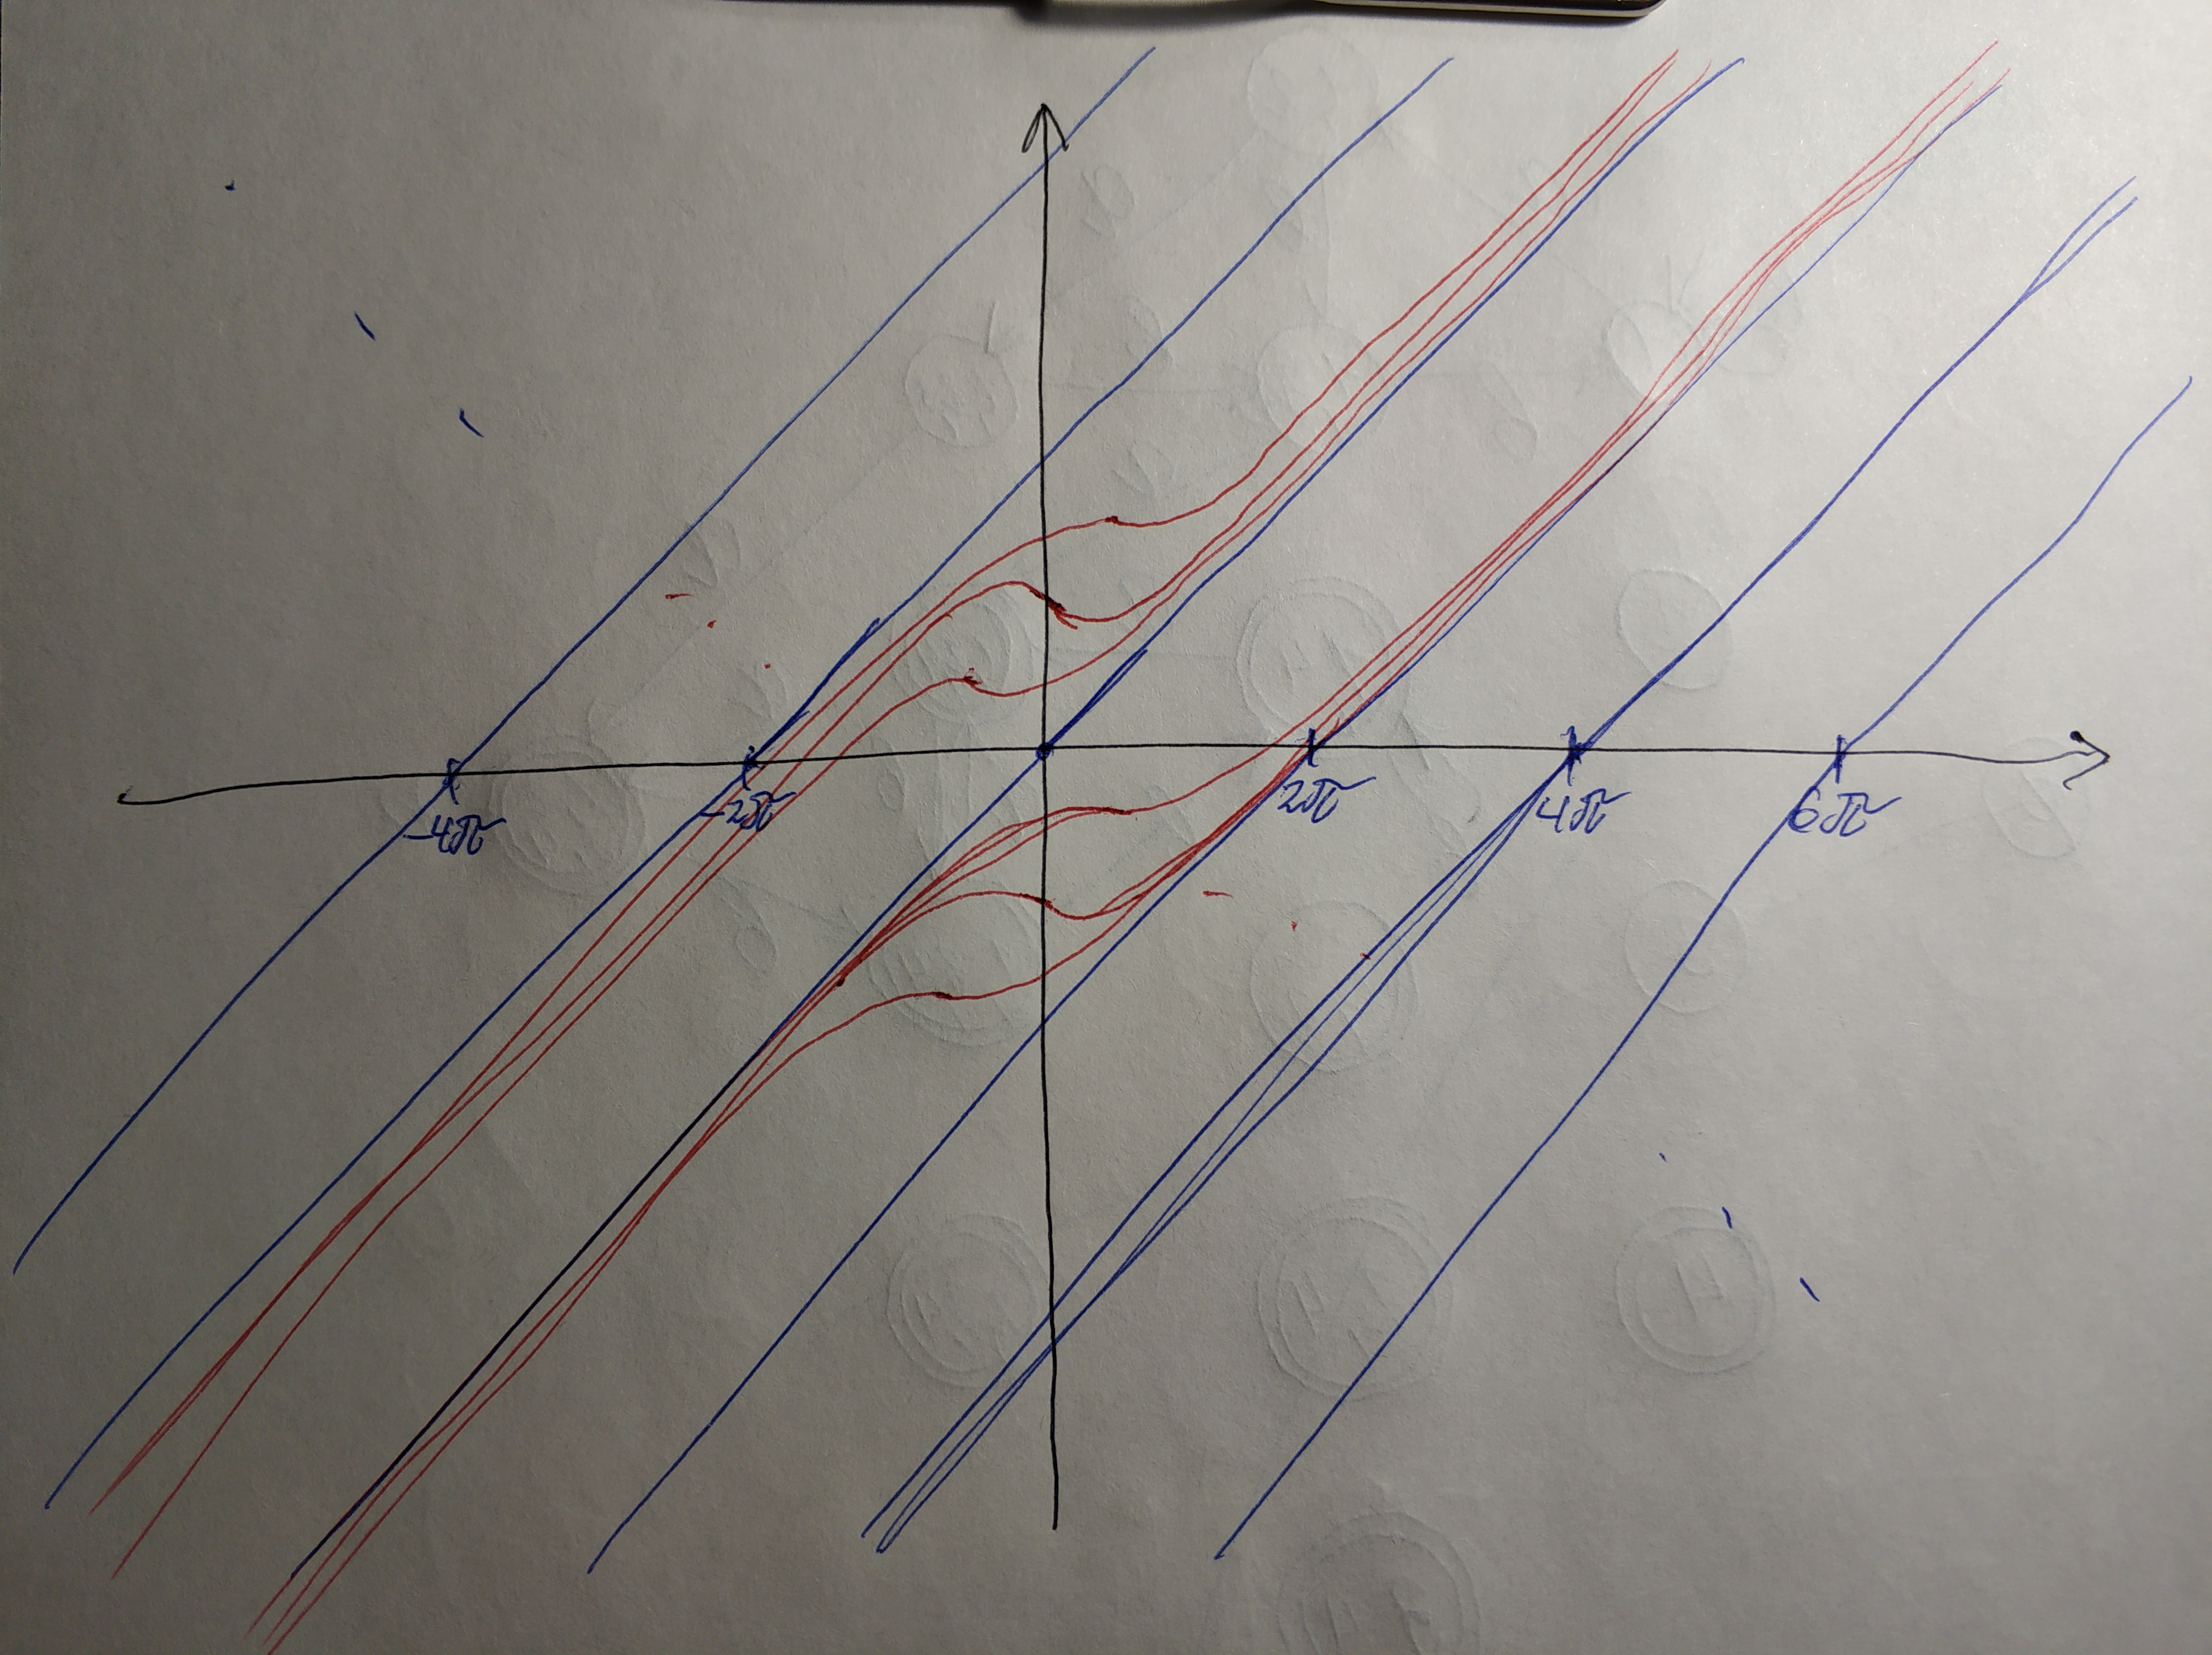
\includegraphics[height=12cm]{DEaDS-HW-002-3.jpg}
        \end{figure}
        Несложно видеть, что из-за константы $n$ область делится на полоски горизонтальной ширины $2\pi$, параллельные прямой $y = x$. А из-за константы $C$ мы имеем расслоение внутри каждой полосы (при этом решения получаются друг из друга сдвигом, параллельным той же прямой $y = x$, или сдвигом на $2\pi n$ по горизонтали).
    \end{problem}
\end{document}